\textbf{9-1.}一质点沿 $x$ 轴做简谐振动, 其运动方程为 $x = 0.4 \cos \left[3 \pi \left(t + \frac{1}{6}\right)\right]$ , 式中 $x$ 和 $t$ 的单位分别为 $\mathbf{m}$ 和 $\mathbf{s}$ 。求:

(1) 振幅、周期和角频率；

(2) 初相位、初位移和初速度；

(3) t=1.5 s 时的位移、速度和加速度。

\vfill

\textbf{9-2.}一质点做振幅 $A = 0.30 \mathrm{~m}$ 的简谐振动。当质点的位移 $x = 0.15 \mathrm{~m}$ 时的速度大小为 $v = 0.9 \mathrm{~m} / \mathrm{s}$ , 求振动频率 $\nu$ 。

\vfill
\newpage

\textbf{9-3.}一质点做正弦简谐振动, 在某相位时, 其位移为 $x_0$ , 当相位增大一倍时, 其位移为 $\sqrt{3} x_0$ 。求振幅 $A$ 。

\vfill

\textbf{9-4.}一根质量为 $m$ 的均匀杆, 放在两个完全相同的轮子上, 两轮心间距离为 $2l$ , 并沿习题 9-4 图 (a) 所示的方向高速旋转, 杆与轮子间的摩擦因数为 $\mu$ , $t = 0$ 时, 杆静止, 杆的质心与两轮中间点的距离为 $x_0$ 。

(1) 证明杆沿水平方向将做简谐振动,并求出振动的角频率;

(2) 若两轮均沿与习题 9-4 图(a)所示的相反方向旋转, 求杆的质心从 $x_{0}$ 运动到任意一点 $x$ ( $x$ 表示杆的质心与两轮中间点的距离)时所用的时间。

\begin{figure}[H]
  \centering
  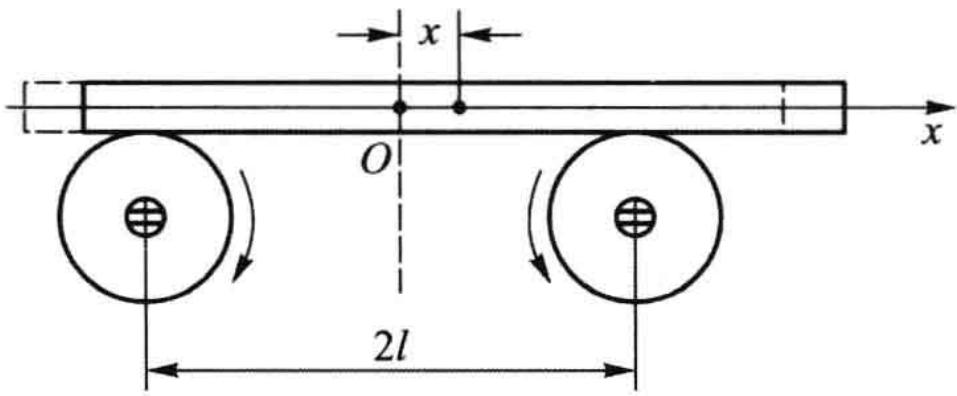
\includegraphics[width=0.4\textwidth]{figures/fig9-4_a.jpg}
  \end{figure}

\vfill
\newpage

\textbf{9-5.}一摆长为 $l$ , 摆锤质量为 $m$ 的单摆悬挂在火车顶上。当火车以加速度 $a_0$ 行驶时,

(1) 求证: 单摆平衡时, 摆线与竖直线之间将有一夹角 $\theta_{0}, \theta_{0}$ 的值为
$$
\theta_ {0} = \arctan \left(\frac {a _ {0}}{g}\right)
$$

(2) 将摆锤偏离平衡位置少许后释放, 求其振动周期。

\begin{figure}[H]
  \centering
  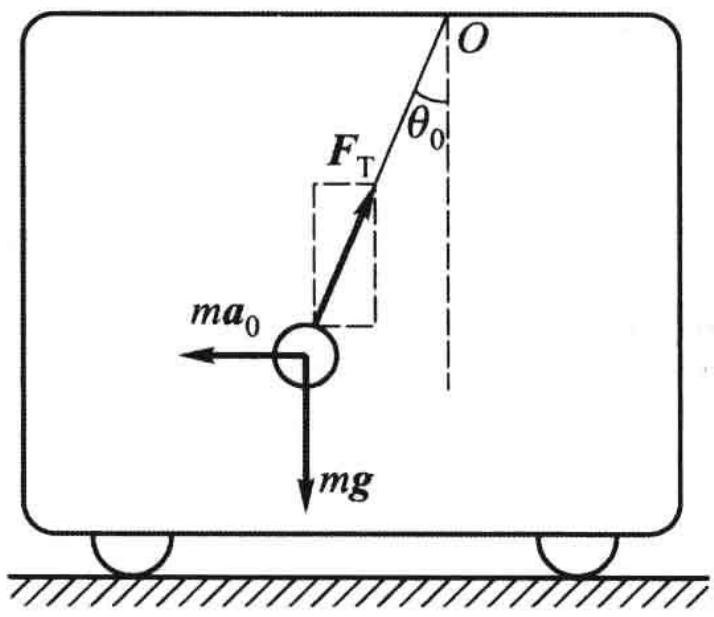
\includegraphics[width=0.25\textwidth]{figures/fig9-5.jpg}
  \end{figure}

\vfill

\textbf{9-6.}若上题中的单摆挂在电梯的顶上。

(1) 若电梯以加速度 $a_0$ 向下运动, 则摆的周期为多大? 若 $a_0 > g$ , 则会出现什么现象?

(2) 若电梯以加速度 $a_0$ 向上运动, 则摆的周期有多大?

\vfill
\newpage

\textbf{9-7.}由一长为 $l$ 、质量为 $m$ 的杆和一质量为 $m_0$ 、半径为 $R$ 的匀质圆盘组成的复摆，如习题9-7图所示。求此复摆在以下两种情况下的周期和等值单摆长。

(1) 圆盘与杆固连；

(2) 圆盘与杆之间由一光滑轴相连, 故圆盘可绕此轴自由旋转。

\begin{figure}[H]
  \centering
  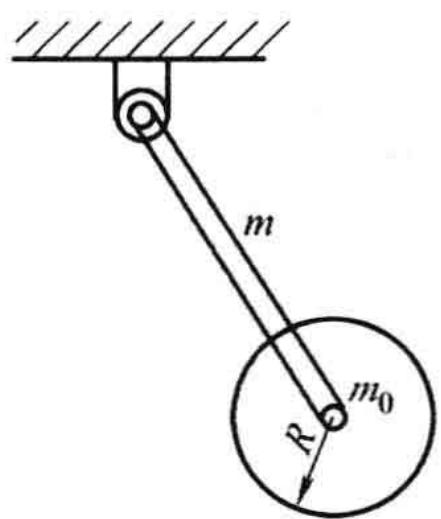
\includegraphics[width=0.25\textwidth]{figures/fig9-7.jpg}
  \end{figure}

\vfill

\textbf{9-8.}一半径为 $R$ 的光滑圆环以恒定的角速度 $\omega$ 绕其竖直的直径旋转, 圆环上套有一小珠。试求:

(1) 小珠相对圆环的平衡位置(以小珠与圆心连线同竖直直径间的夹角 $\theta_{0}$ 表示);

(2) 小珠在平衡位置附近做小振动的角频率。

\begin{figure}[H]
  \centering
  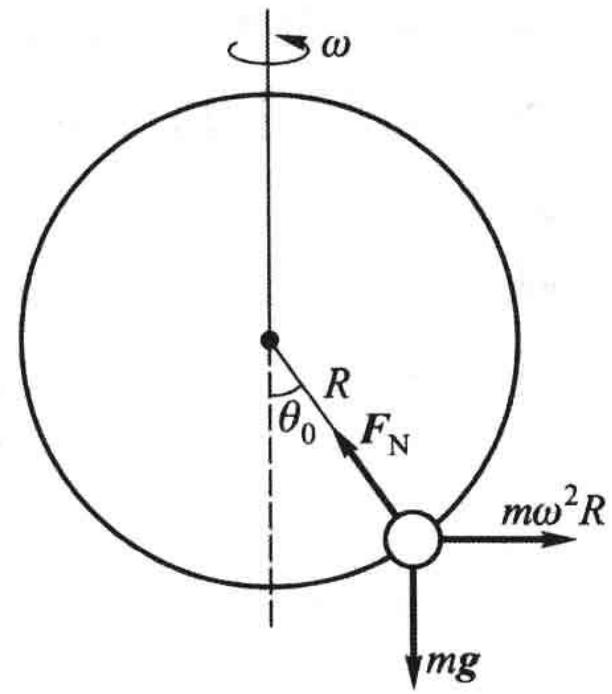
\includegraphics[width=0.25\textwidth]{figures/fig9-8.jpg}
  \end{figure}

\vfill
\newpage

\textbf{9-9.}如在质量均匀分布的球形行星上沿任一直径挖一隧道。将一物体由静止开始从一道口自由掉下。

(1) 求证物体到达隧道的另一道口所需的时间与物体的质量无关,与行星的直径无关,只与行星的密度 $\rho$ 有关,并计算该时间;

(2) 若隧道是沿行星的任一弦挖的, 求证该时间与弦的长短、位置均无关, 并证明该时间与(1)中的完全一样;

（3）若行星以角速度 $\omega_0\left(\omega_0 < \sqrt{\frac{4\pi\rho G}{3}}\right)$ 匀速自旋，角速度方向与隧道垂直，则(1)、(2)中的时间又为多大？

(4) 若上述行星为地球, 已知地球密度 $\rho_{0} = 5.52 \times 10^{3} \mathrm{~kg} / \mathrm{m}^{3}, G = 6.67 \times 10^{-11} \mathrm{~N} \cdot \mathrm{m}^{2} / \mathrm{kg}^{2}$ 。由于地球自旋角速度很小, 故可忽略。试计算 (1)、(2) 两问中所提及的时间。

\begin{figure}[H]
  \centering
  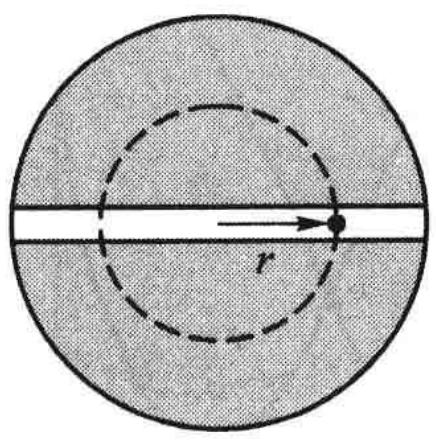
\includegraphics[width=0.2\textwidth]{figures/fig9-9.jpg}
  \end{figure}

\vfill

\textbf{9-10.}两个同方向同频率的简谐振动 $x_{1} = 0.4\cos \left(0.5\pi t + \frac{\pi}{6}\right)(\mathrm{m}), x_{2} = 0.2\cos (0.5\pi t + \varphi_{2})(\mathrm{m})$ ，试问：

(1) $\varphi_{2}$ 为何值时合振动的振幅最大？并求出此振幅值。

(2) 若合振动的初相位 $\varphi = \varphi_{2} + \frac{\pi}{2}$ ，则 $\varphi_{2}$ 为何值？

\vfill
\newpage

\textbf{9-11.}一架钢琴的“中音 C”有些不准,出于校准的需要,另取一架标准的钢琴,同时弹响这两架钢琴的“中音 C”键,在 1 分钟内听到 24 拍。试求待校准钢琴此键音的频率。

\vfill

\textbf{9-12.}两个互相垂直的振动表达式为:

$$
x = 3 \cos (2 \pi t), y = 3 \cos \left(4 \pi t + \frac {\pi}{3}\right)
$$

试作出合振动的轨迹图。

% \begin{figure}[H]
%   \centering
%   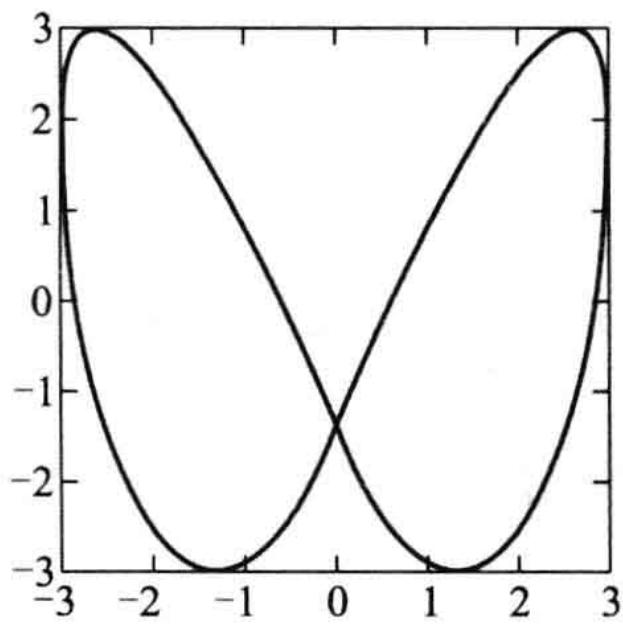
\includegraphics[width=0.4\textwidth]{figures/fig9-12.jpg}
%   \end{figure}

\vfill
\newpage


\textbf{9-13.}一根杆与竖直轴固连, 两者之间成 $\theta$ 角, 一根劲度系数为 $k$ , 原长为 $l_{0}$ 的弹簧套在杆上, 其一端与竖直轴相连, 另一端系一个同样套在杆上的质量为 $m$ 的小圆环,如习题9-13图所示。开始时杆以恒定的角速度 $\omega$ 绕竖直轴旋转,小圆环相对杆静止。

(1) 求此时小圆环的位置 $x_{0}$ ;

(2) 若转动角速度突然变为 $2 \omega$ , 则小圆环从位置 $x_{0}$ 运动到离轴最远处所需的时间 $t$ 为多大?

\begin{figure}[H]
  \centering
  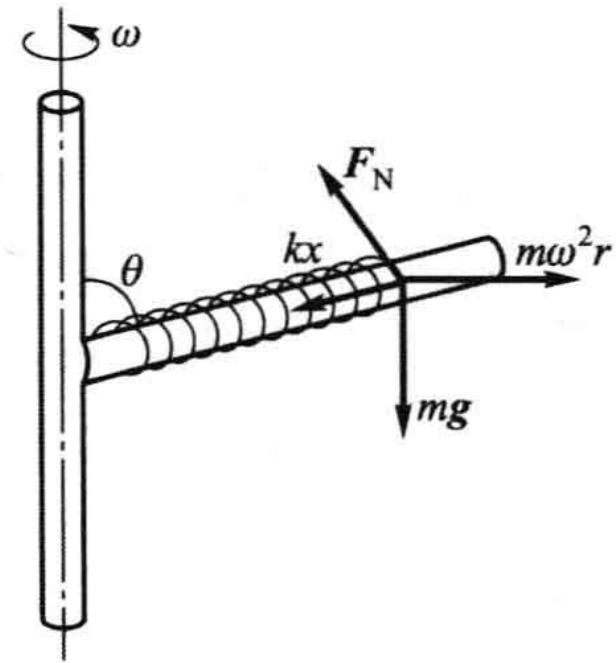
\includegraphics[width=0.25\textwidth]{figures/fig9-13.jpg}
  \end{figure}

\vfill

\textbf{9-14.}如习题 9-14 图所示, 在光滑的水平桌面上开有一小孔, 一条穿过小孔的细绳两头各系一质量分别为 $m_{1}$ 和 $m_{2}$ 的小球, 位于桌面上的小球 $m_{1}$ , 以 $v_{0}$ 的速度绕小孔做匀速圆周运动, 而小球 $m_{2}$ 则悬在空中, 保持静止。

(1) 求位于桌面部分的细绳的长度 $l_{0}$ ;

(2) 若给 $m_{1}$ 一微小的径向冲量, 则 $m_{2}$ 将做上下小振动, 求振动角频率 $\omega_{0}$ 。

\begin{figure}[H]
  \centering
  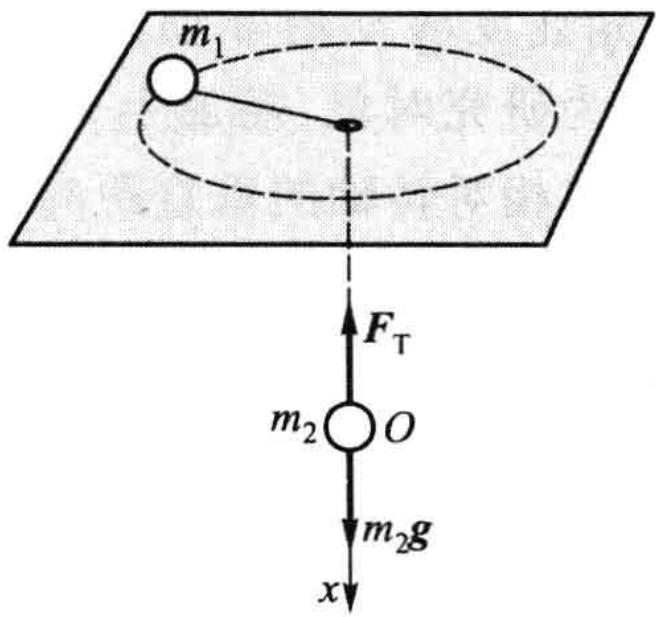
\includegraphics[width=0.25\textwidth]{figures/fig9-14.jpg}
  \end{figure}

\vfill
\newpage

\textbf{9-15.}一质量为 $m$ 、边长为 $a$ 的正三角形薄板, 通过其某一角悬挂在与板面垂直的光滑水平轴上, 构成一复摆。求此复摆的周期和等值单摆长。

\begin{figure}[H]
  \centering
  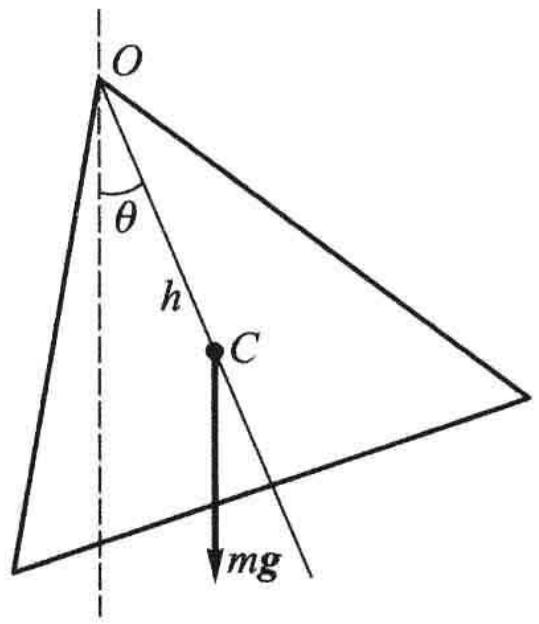
\includegraphics[width=0.2\textwidth]{figures/fig9-15_a.jpg}
  \end{figure}

\vfill

\textbf{9-16.}质量为 $m_{0}$ 的小球和长为 $l$ 、质量为 $m$ 的杆组成的复摆, 被刚性地固定在一横轴上, 而横轴被架在一平台上的两个支架上, 如习题 9-16 图所示。当平台以较小的角速度 $\Omega$ 绕其中心轴(通过摆的上端)旋转时,求该复摆的振动周期,设小球的半径可忽略。

\begin{figure}[H]
  \centering
  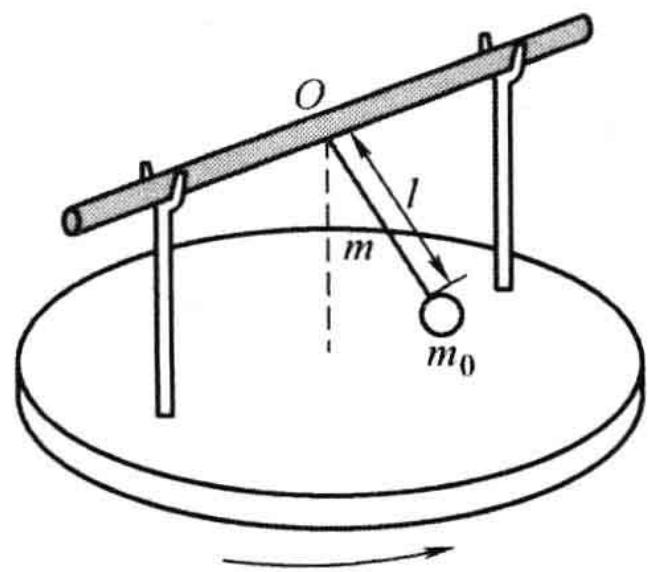
\includegraphics[width=0.2\textwidth]{figures/fig9-16.jpg}
  \end{figure}

\vfill
\newpage

\textbf{9-17.}如习题 9- 17 图所示,一深水池中竖立着一根光滑的细杆,一长度为 $L$ 的匀质细管套在杆上。用手持管,使其下端正好与水面接触,然后放手,设水的密度为 $\rho_{0}$ 。

(1) 若管运动到最低位置时, 其上端正好与水面持平, 求管的密度 $\rho_{1}$ ;

(2) 证明在(1)中情况下,细管将做简谐振动,求出振幅和周期;

(3) 若管的密度为 $\frac{4}{3} \rho_{1}$ , 求管下沉到最低位置所需的时间。

\begin{figure}[H]
  \centering
  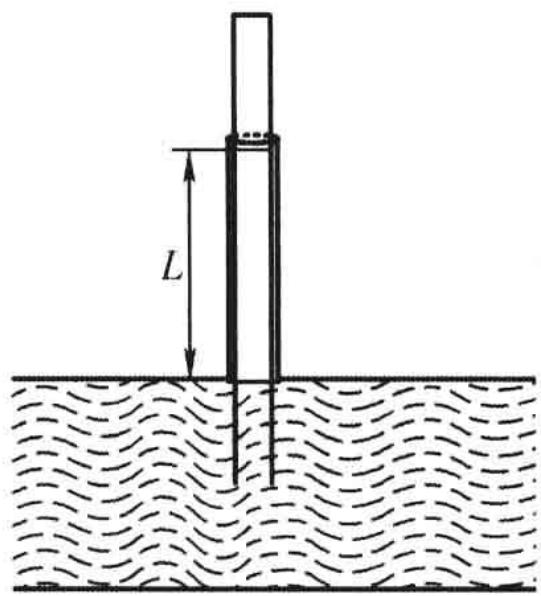
\includegraphics[width=0.25\textwidth]{figures/fig9-17.jpg}
  \end{figure}

\vfill

\textbf{9-18.}试作出下列两振动的合振动的李萨如图：

(1) $x = \cos \omega t, y = \cos 2\omega t$ 。

(2) $x = \cos 2\omega t, y = \cos (3\omega t + \pi)$ 。

% \begin{figure}[H]
%   \centering
%   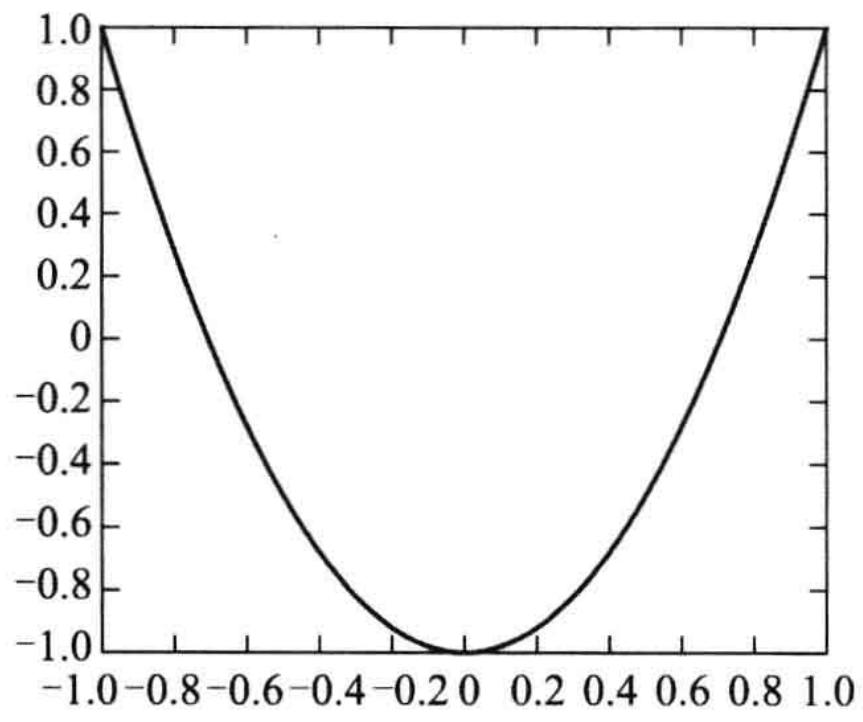
\includegraphics[width=0.4\textwidth]{figures/fig9-18_a.jpg}
%   \end{figure}

\vfill
\newpage

\textbf{9-19.}一质量为 $m_{0}$ 的物块置于一光滑水平面上, 物块的两端各系有一弹簧, 弹簧的自然长度均为 20 cm, 其劲度系数分别为 $k_{1}$ 与 $k_{2}$ 。现将两弹簧分别与两壁相连, 两壁与两弹簧原来的自由端都相距 10 cm, 如习题 9-19 图所示。设 $k_{1}=1\ N/m, k_{2}=3\ N/m, m_{0}=100\ g$ 。

(1) 当物块处于平衡位置时, 求每个弹簧的长度;

(2) 若将此物块略微偏离平衡位置后释放,试求其振动周期;

(3) 设此物块振动的振幅为 $5 \mathrm{~cm}$ , 当其通过平衡位置时, 有一质量为 $m = 100 \mathrm{~g}$ 的泥灰竖直地落于其上, 并与之一起运动, 试求此系统的振动周期和振幅;

(4) 若(3)中的泥灰在物块运动到最大位移处时落于其上,求这种情况下系统振动的周期和振幅。

\begin{figure}[H]
  \centering
  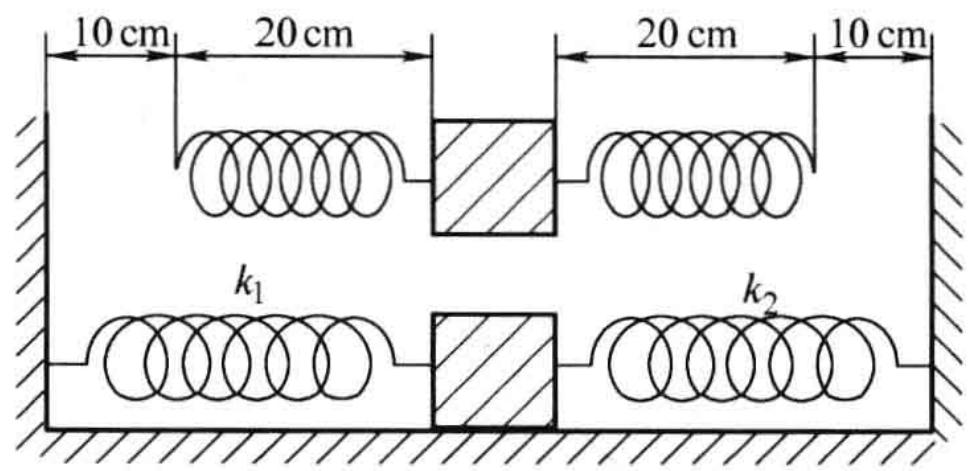
\includegraphics[width=0.3\textwidth]{figures/fig9-19_2.jpg}
  \end{figure}

\vfill

\textbf{9-20.}如习题 9-20 图所示, 一弹簧振子, 其质量 $m_{1} = 98 \mathrm{~g}$ , 劲度系数 $k_{1} = 9.8 \times 10^{-2} \text{ N/cm}$ , 它的影子水平地投射到一质量 $m_{2} = 980 \text{ g}$ 的屏上, 屏在一劲度系数 $k_{2} = 0.98 \text{ N/cm}$ 的弹簧下。开始时把两者都从平衡位置拉下 $10 \text{ cm}$ , 先释放弹簧振子使之振动。如果要使影子在屏上振动的振幅为 $5 \text{ cm}$ , 试问应隔几秒钟后释放屏使之振动? 并写出此时影子在屏上的振动方程。

\begin{figure}[H]
  \centering
  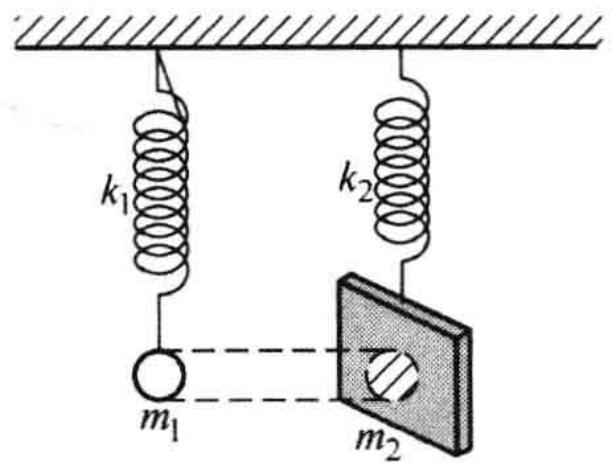
\includegraphics[width=0.3\textwidth]{figures/fig9-20.jpg}
  \end{figure}

\vfill
\newpage

\textbf{9-21.}一面积为 $S$ 、质量为 $m$ 的薄板连在弹簧的下端, 弹簧的上端固定, 薄板浸在黏性液体中,如习题9-21图所示。设薄板在黏性液体中受到的阻力 $F_{f}=-2\mu Sv$ ,式中v为薄板在竖直方向上的运动速度, $\mu$ 是一个与液体黏性有关的常量。设此系统的振动周期为T,求此系统在空气中时的振动周期 $T_{0}$ 。

\begin{figure}[H]
  \centering
  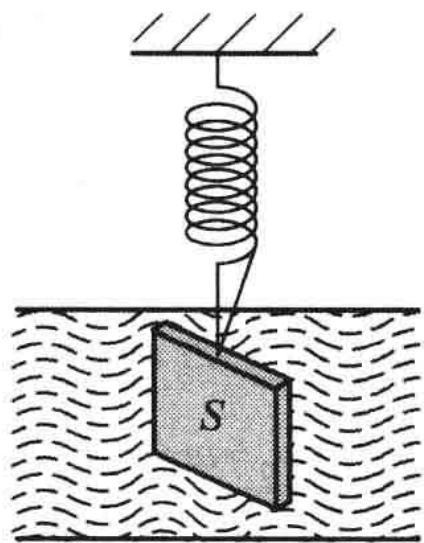
\includegraphics[width=0.25\textwidth]{figures/fig9-21.jpg}
  \end{figure}

\vfill

\textbf{9-22.}一质量为 $0.2 \mathrm{~kg}$ 的物体, 悬于颈度系数为 $10 \mathrm{~N} / \mathrm{m}$ 的弹簧下, 此物体受到的阻力 $F_{\mathrm{f}} = -b v$ , 其中 $v$ 是物体的速度 (单位是 $\mathrm{m} / \mathrm{s}$ ), $b$ 为一较小的常量。

(1) 写出系统振动的运动方程;

(2) 若系统振动频率比无阻尼时小了万分之一, 即 $\frac{\omega_0 - \omega_f}{\omega_0} = 10^{-4}$ , 则常量 $b$ 为多大?

(3) 此系统的 $Q$ 值为多大? 振动经一个整周期后, 振幅减弱为几分之几?

\vfill
\newpage

\textbf{9-23.}某阻尼振动的振幅在一个周期后减为原来的 $1 / 4$ , 问此振动周期比无阻尼存在时的周期大百分之几?

\vfill

\textbf{9-24.}一摆长为 $l = 0.750 \mathrm{~m}$ 的单摆做阻尼振动, 经过一分钟后, 其振幅衰减为开始时的 $1 / 8$ , 求对数减缩 $\lambda$ (即 $\lambda = \delta T$ )。

\vfill
\newpage

\textbf{9-25.}某振动系统从开始振动,经过16次振动后,能量减为开始时的0.6。问再经过16次振动后,系统能量减为开始时的几分之几?

\vfill

\textbf{9-26.}当在某钢琴上弹响“中音 C”这个琴键时, 其振动能量在 $1 \mathrm{~s}$ 内减至初始值的一半。已知中音 C 的频率为 $256 \mathrm{~Hz}$ 。求此系统的 Q 值。

\vfill
\newpage

\textbf{9-27.}一质量为 $10 \mathrm{~kg}$ 的物体, 从 $0.5 \mathrm{~m}$ 高处静止下落到弹簧秤的秤盘里, 并黏附在盘上。已知秤盘的质量为 $2.0 \mathrm{~kg}$ , 弹簧的劲度系数为 $980 \mathrm{~N} / \mathrm{m}$ 。为使秤盘在最短时间内停下来, 就须附上一阻尼系统。求出所必需的阻尼因数 $\delta$ , 并写出秤盘的位置 $y$ 随时间 $t$ 的变化关系 ( $y$ 的零点取在平衡位置, $t$ 的零点取在物体掉在秤盘的瞬间)。

\vfill

\textbf{9-28.}摆长为 $1 \mathrm{~m}$ 的单摆, 在振动 50 次后振幅减为原来的 $\frac{1}{\mathrm{e}}$ 。现使其悬点做振幅为 $1 \mathrm{~mm}$ 的水平方向上的简谐振动。

(1) 若摆锤的水平位移为 $x_{1}$ , 悬点的水平位移为 $x_{2}$ , 试证明摆锤做微小振动时的运动方程为 $\frac{\mathrm{d}^{2} x_{1}}{\mathrm{d} t^{2}} + 2 \delta \frac{\mathrm{d} x_{1}}{\mathrm{d} t} + \frac{g}{l} x_{1} = \frac{g}{l} x_{2}$ 。如果 $x_{2} = A \cos \omega t$ , 试求此方程的稳态解。

(2) 求共振时摆锤运动的振幅。

(3) 在什么角频率时, 其振幅为共振时的一半?

\begin{figure}[H]
  \centering
  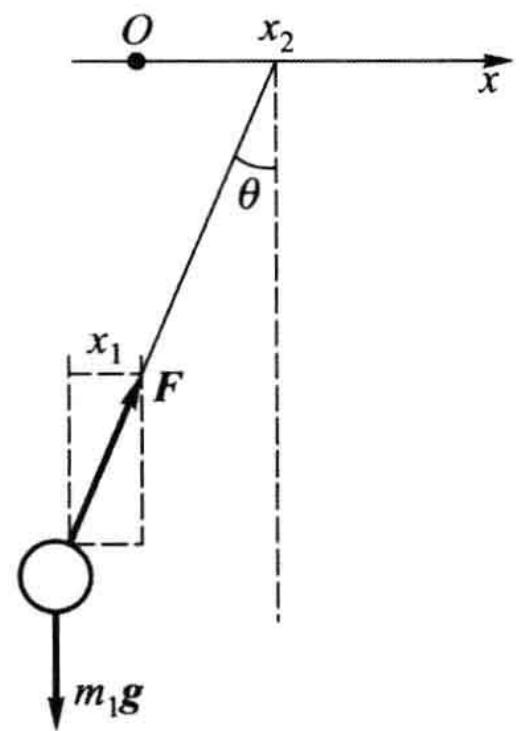
\includegraphics[width=0.23\textwidth]{figures/fig9-28.jpg}
  \end{figure}

\vfill
\newpage

\textbf{9-29.}一谐振子质量 $m = 0.10 \mathrm{~kg}$ , 做周期 $T = 2.5 \mathrm{~s}$ 的简谐振动, 质点振动的总能量 $E = 0.20 \mathrm{~J}$ , 求作用在质点上力的最大值。

\vfill

\textbf{9-30.}一物体悬挂于弹簧下,系统固有振动周期为 $0.50 \mathrm{~s}$ ,今在物体上加一竖直方向的余弦力,其最大值 $F = 1 \times 10^{-3} \mathrm{~N}$ ;此外物体还受到一摩擦阻力 $F_{\mathrm{f}} = -C \dot{x}$ 作用, $C$ 为一较小的常量。已知系统在共振时的振幅为 $5.0 \mathrm{~cm}$ ,求物体在运动过程中受到的最大摩擦力的数值 $F_{\mathrm{f,max}}$ 。

\vfill
\newpage

\textbf{9-31.}做受迫振动的振子, 若其速度与强迫力同相位, 求强迫力的频率。设振子的固有频率为 $\omega_{0}$ 。

\vfill

\textbf{9-32.}一振子在强迫力 $F = F_{0} \cos \omega t$ 的驱动下做受迫振动。已知振子的质量 $m = 0.2 \mathrm{~kg}$ ，弹簧的劲度系数 $k = 80 \mathrm{~N} / \mathrm{m}$ ，阻力系数 $C = 4 \mathrm{~N} \cdot \mathrm{s} / \mathrm{m}$ ，若 $F_{0} = 2 \mathrm{~N}$ ， $\omega = 30 \mathrm{~s}^{-1}$ 。试问：

(1) 振子系统在一周内反抗阻力而耗散的能量是多少?

(2) 输入系统的平均功率是多少?

\vfill
\newpage

\textbf{9-33.}某振动系统的固有频率为 $1000 \mathrm{~Hz}$ , 品质因数为 50, 若其共振时驱动力所提供的平均功率为 $5.0 \mathrm{~mW}$ , 求此时振子的能量。

\vfill

\textbf{9-34.}习题 9-34 图所示为某振动系统在驱动力 $F = F_{0} \sin \omega t$ 的驱动下的平均功率共振曲线。此处 $F_{0}$ 是常量。

(1) 求出此系统的固有频率 $\omega_{0}$ 和品质因数 Q 的数值；

(2) 若撤去驱动力, 则系统经过多少周后能量降至初始值的 $e^{-5}$ ?

\begin{figure}[H]
  \centering
  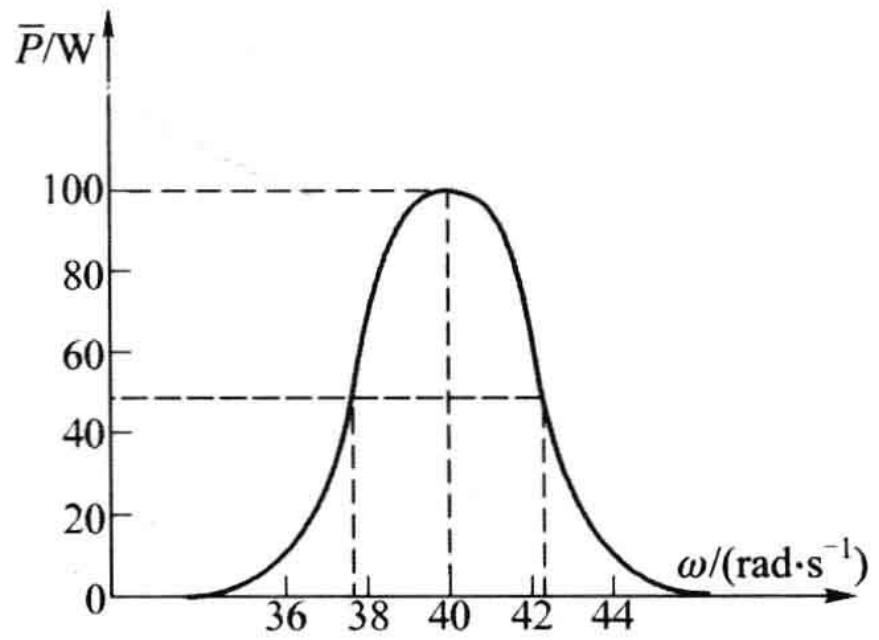
\includegraphics[width=0.4\textwidth]{figures/fig9-34.jpg}
  \end{figure}

\vfill
\newpage

\textbf{9-35.}两个质量都为 $m$ 的质点, 如习题 9-35 图连接在三个劲度系数都是 $k$ 的弹簧上, 两质点间连接一质量可以忽略的阻尼减震器, 阻尼减震器所施的力为 $bv$ , 这里 $v$ 是它两端的相对速度, $b$ 为常量。该力阻止其两端之间 (即两质点之间) 的相对运动。令 $x_{1}, x_{2}$ 分别为两质点离开其平衡位置的位移。

(1) 写出每个质点的运动方程；

(2) 证明运动方程可以用新的变量 $y_{1} = x_{1} + x_{2}$ 和 $y_{2} = x_{1} - x_{2}$ 来求解；

(3) 证明: 如果两质点原来静止于平衡位置, 在 $t = 0$ 时给质点 1 以初速度 $v_{0}$ , 则在足够长的时间以后, 两个质点的运动方程为 $x_{1} = x_{2} = \frac{v_{0}}{2 \omega} \sin \omega t$ , 并求出 $\omega$ 。

\begin{figure}[H]
  \centering
  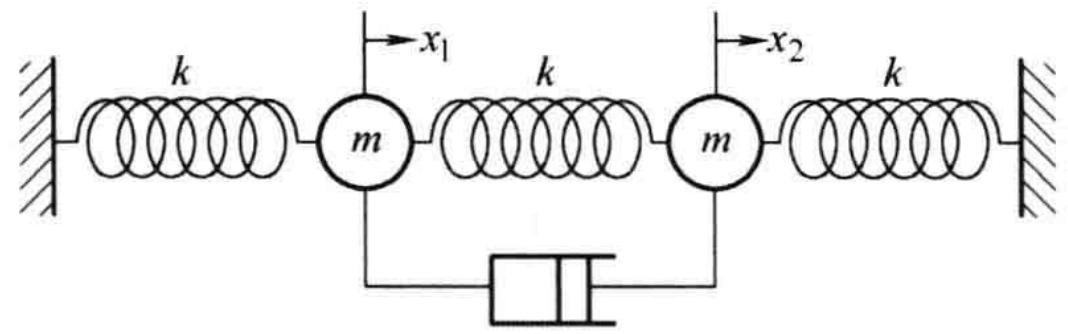
\includegraphics[width=0.4\textwidth]{figures/fig9-35_1.jpg}
  \end{figure}

\vfill

\textbf{9-36.}由劲度系数为 $k$ 的轻弹簧和质量为 $m$ 的质点构成的两个相同弹簧振子串联地竖直悬挂, 求此系统沿竖直方向做振动的简正频率。

\begin{figure}[H]
  \centering
  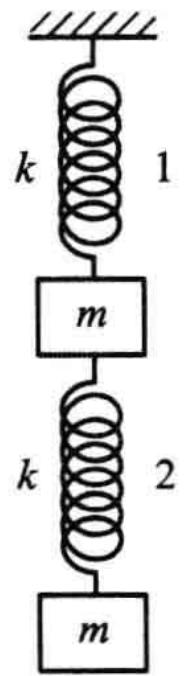
\includegraphics[width=0.08\textwidth]{figures/fig9-36.jpg}
\end{figure}

\vfill
\newpage
